\newcommand{\institut}{Institut f\"ur Telekommunikationssysteme}
\newcommand{\fachgebiet}{Nachrichten\"ubertragung}
\newcommand{\veranstaltung}{Praktikum Nachrichten\"ubertragung}
\newcommand{\pdfautor}{Dirk Babendererde (321 836), Thomas Kapa (325 219)}
\newcommand{\autor}{Dirk Babendererde (321 836)\\ Thomas Kapa (325 219)}
\newcommand{\gruppe}{Gruppe:}
\newcommand{\betreuer}{Betreuer: Lieven Lange}


\newcommand{\pdftitle}{Nachrichtenuebertragung\ Praktikum\ 05}
\newcommand{\prototitle}{Praktikum 05 \\ Pulsamplitudenmodulation und nichtideale Abtastung}

\input{../../packages/tu_header_9}

% damit das outline funktioniert noch mal:
\begin{document}


%     \lstinputlisting{./praktikum6.sce}

%---------------------------------------------------------------------
%---------------------------------------------------------------------
%---------------------------------------------------------------------

\section{Vorbereitung}
\begin{quote}
    
    
    \begin{figure}[H]
        \centering
        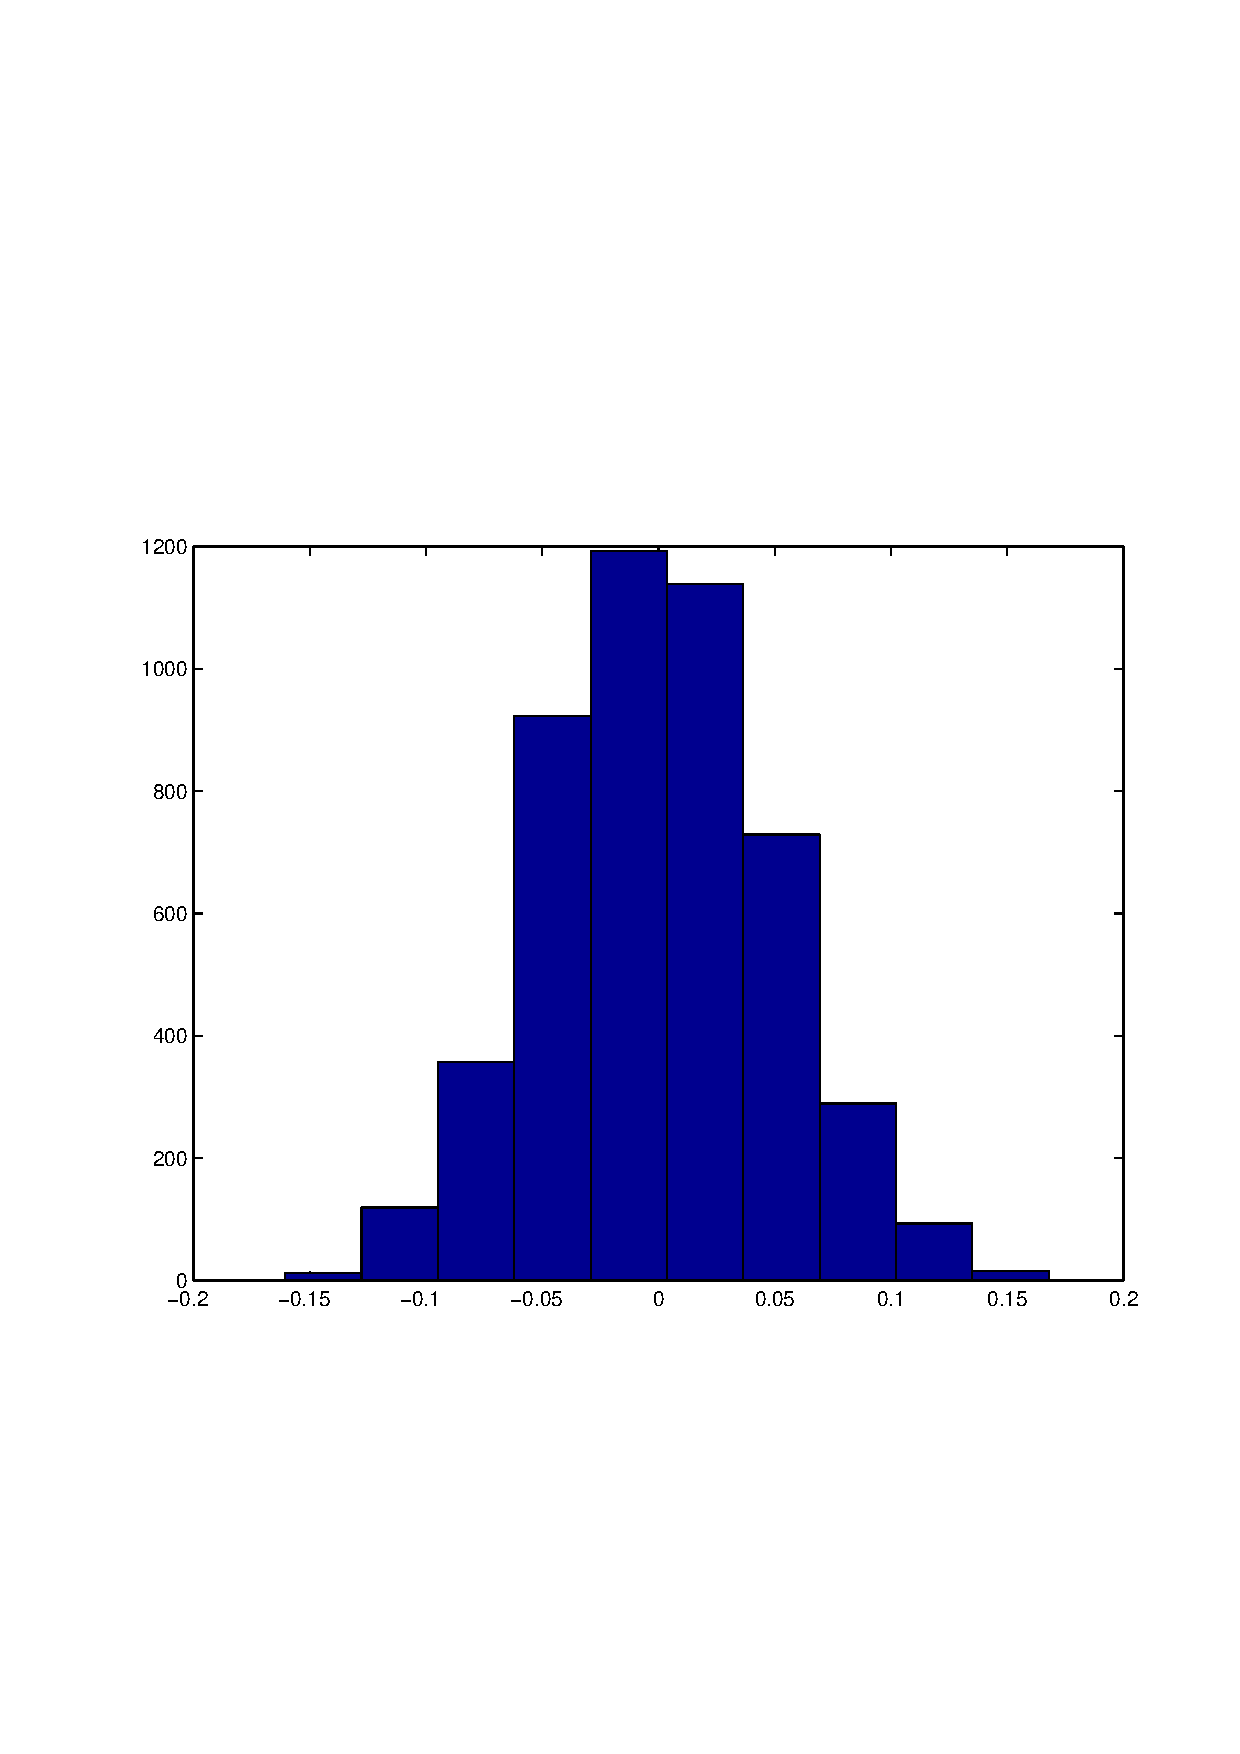
\includegraphics[scale=0.7, trim = 2cm 7cm 1cm 8cm, clip]{Bilder/PCM_Test}
        \caption{Testkennlinie des PCM-Analyse Scriptes}
        \label{fig:PCM_Test}
    \end{figure}
    
    
    \TODO{Blockschaltbild? erklärung?}
    
    
    
    
\end{quote}


\section{Labordurchführung}
\begin{quote}


	\subsection{Encoderkennlinie}
		\begin{quote}
		
			Es soll die PCM-Encoder-Kennlinie aufgenommen werden.
			Dazu wird das PCM-Encoder-Modul des ETT101 genutzt. Zunächst wird als Clocksignal an den Eingang CLK das 
			100 kHz DIGITAL Signal des Master Signals-Modul gelegt. Anschließend wird als Eingang in INPUT 1 ein 
			symmetrisches Dreiecksignal mit einer Amplitude von 2,5 Volt angelegt (2,5 Volt, damit für über 2 und unter -2 Volt
			die Codewörter 1111 1111 und 0000 0000 ausgegeben werden) und der Schalter auf PCM gestellt.
			Die beiden Ausgänge FS (Rahmensignal) und PCM (Pulsecode) werden auf die beiden Eingänge des Addierers gegeben. Da
			beide Signale 5 Volt high und 0 Volt low ausgeben, wird die Verstärkung für das PCM-Signal auf 0 gestellt und die
			Verstärkung für das Rahmensignal auf 8/5 gestellt, um die Anforderungen aus der Aufgabenstellung zu erfüllen.
			Mit dem Picoscope werden die Summe aus Rahmensignal und Pulscodesignal und eine steigende Flanke des Zeitignals
			gemessen und angezeigt.
			
			 
		\end{quote}
		
	\subsection{Quantisierungsfehler, Kodieren, Dekodieren}
	
		\begin{quote}
			
			Um den Quantisierungsfehler bestimmen zu können, werden das Eingangssignal und das dekodierte Signal benötigt. Zur
			Dekodierung wird das PCM Decoder-Modul genutzt. Die Eingänge FS, PCM DATA un CLK werden mit ihren jeweiligen
			Gegenstücken des PCM Encoder-Moduls verbunden. Anschließend kann das Signal am OUTPUT 1 zusammen mit dem
			Eingangsignal dem Picoscope zugeführt.\\
			  
			
			
		
		
		\end{quote}
	
	
	 

\end{quote}

\section{Auswertung \& Theorie}
\begin{quote}
    
    \subsection{Encoderkennlinie}
    	
    	\begin{quote}
	   	dsf
    
    	\end{quote}
    	
    	
    \subsection{Quantisierungfehler}
    
    	\begin{quote}
    	Das Signal besitzt in dieser Form noch einen Mittelwert (Offset), welcher mit der Funktion mean in Matlab ermittelt
    	werden kann und vom Signal abgezogen wird. Da weiterhin das Signal durch den Kodier- und Dekodiervorgang eine
    	Dämpfung und einen Delay erfährt, wird das dekodierte Signal mit Hilfe von Matlab verstärkt und mit der Kreuzkorrelation 
    	um die erfahrene Verzögerung verschoben. Das Ergebnis ist in Abb.
    	\ref{fig:100kHz_sin_rek_angepasst} zu sehen. \\
    	
    	\begin{center}
            \begin{tabular}{ll}
            
            \hspace{-5cm}
                \begin{minipage}{0.6\textwidth}
                    \begin{figure}[H]
                        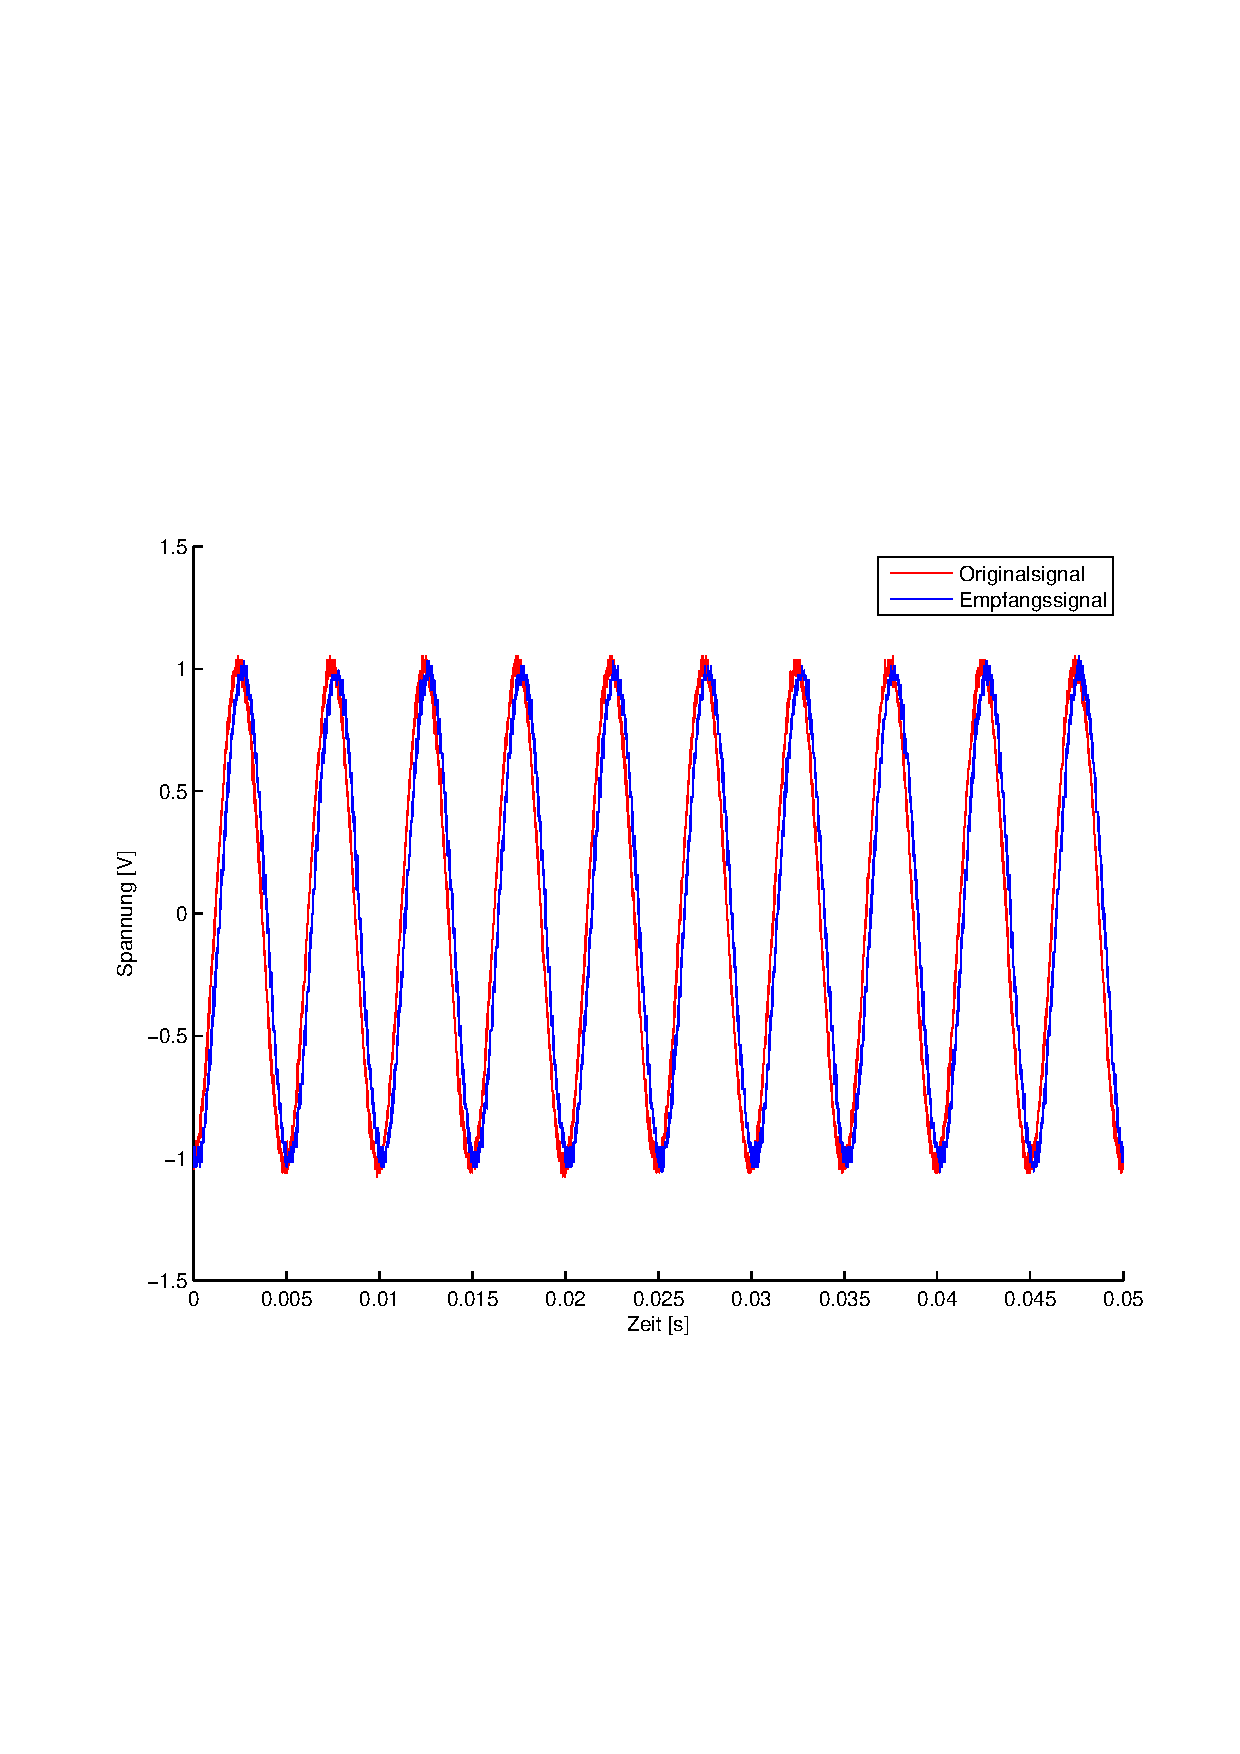
\includegraphics[scale=0.55, trim = 16mm 70mm 16mm 85mm, clip]{Bilder/100kHz_sin_Signal_Rekonstuiert}
                          \caption{100 kHz Sinus noch verschoben}
		                  \label{fig:100kHz_sin_rek}
                    \end{figure}
                \end{minipage}
                
                \begin{minipage}{0.6\textwidth}
                    \begin{figure}[H]
                        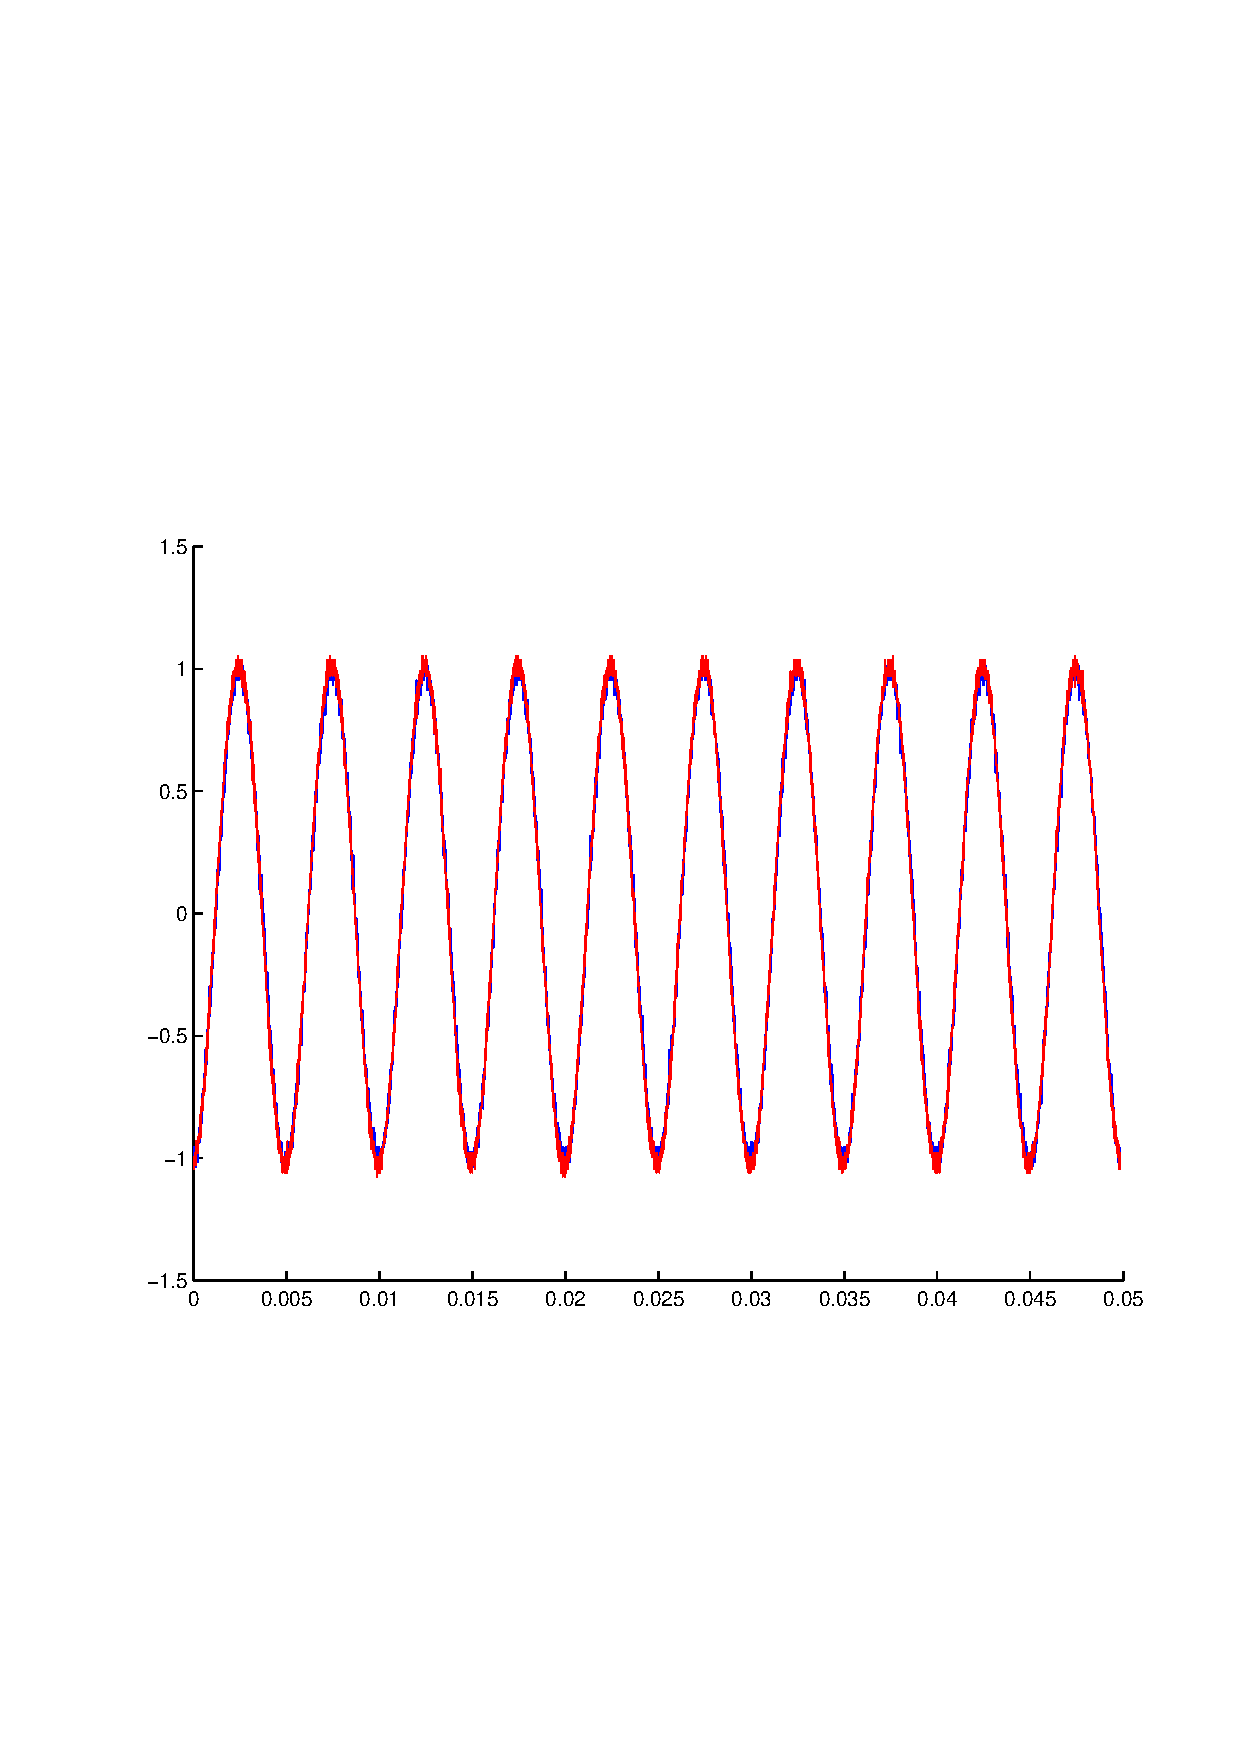
\includegraphics[scale=0.55, trim = 16mm 70mm 16mm 85mm, clip]{Bilder/100kHz_sin_Signal_Rekonstuiert_delayed}
                       \caption{100 kHz Sinus angepasst}
		              \label{fig:100kHz_sin_rek_angepasst}
                    \end{figure}
                \end{minipage}
            
            \end{tabular}
        \end{center}
            
        \vspace{2em}
    	
%     	 \begin{figure}[H]
%             \centering
%             \hspace{-3em}
%             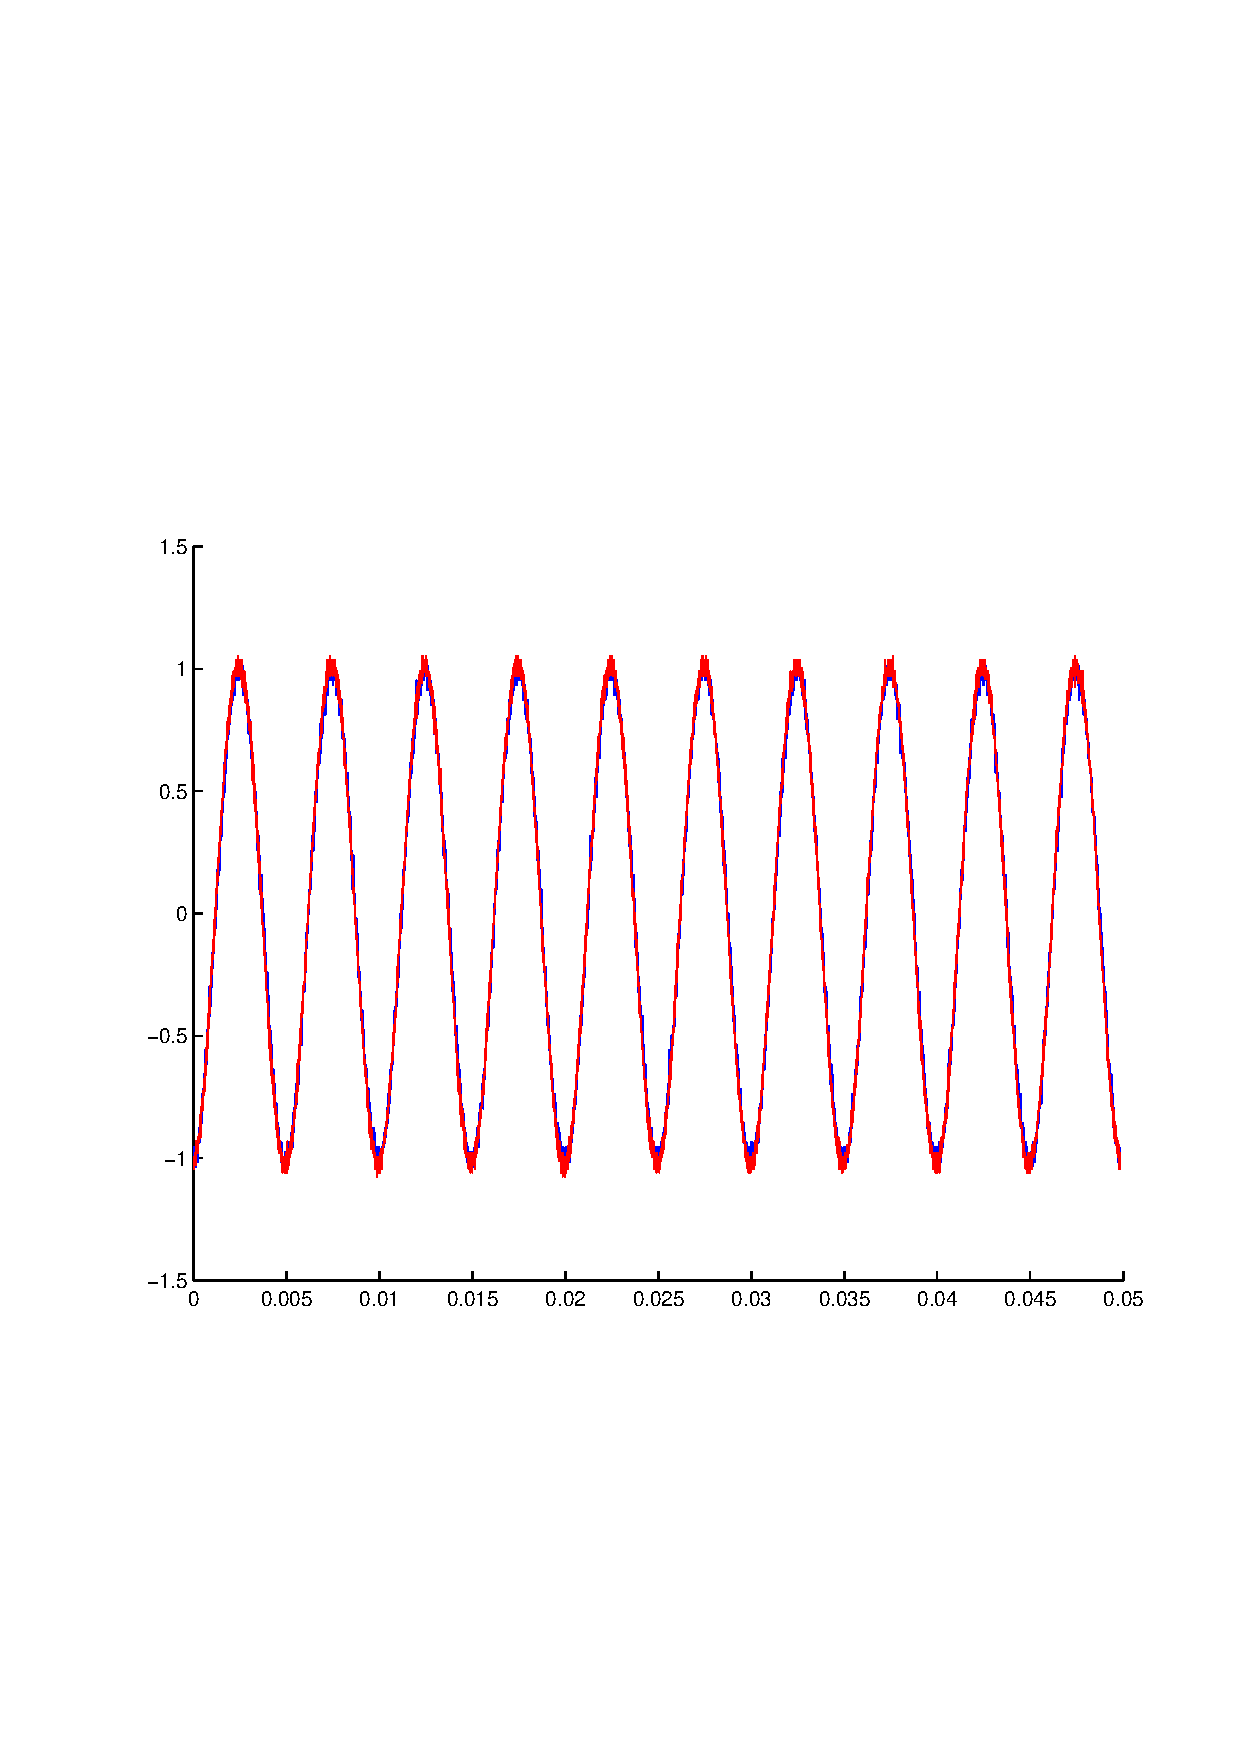
\includegraphics[scale=0.8, trim = 2cm 7cm 1cm 8cm, clip]{Bilder/100kHz_sin_Signal_Rekonstuiert_delayed}
%             \caption{100 kHz Sinus }
%             \label{fig:100kHz_sin_rek_angepasst}
%         \end{figure}
     	
    	
    	
	   	Anschließend können Sendesignal und dekodiertes Signal voneinander subrahiert werden und man erhält den
	   	Quantisierungsfehler.\\
	   	
	   	\begin{center}
            \begin{tabular}{ll}
            
            \hspace{-5cm}
                \begin{minipage}{0.6\textwidth}
                    \begin{figure}[H]
                        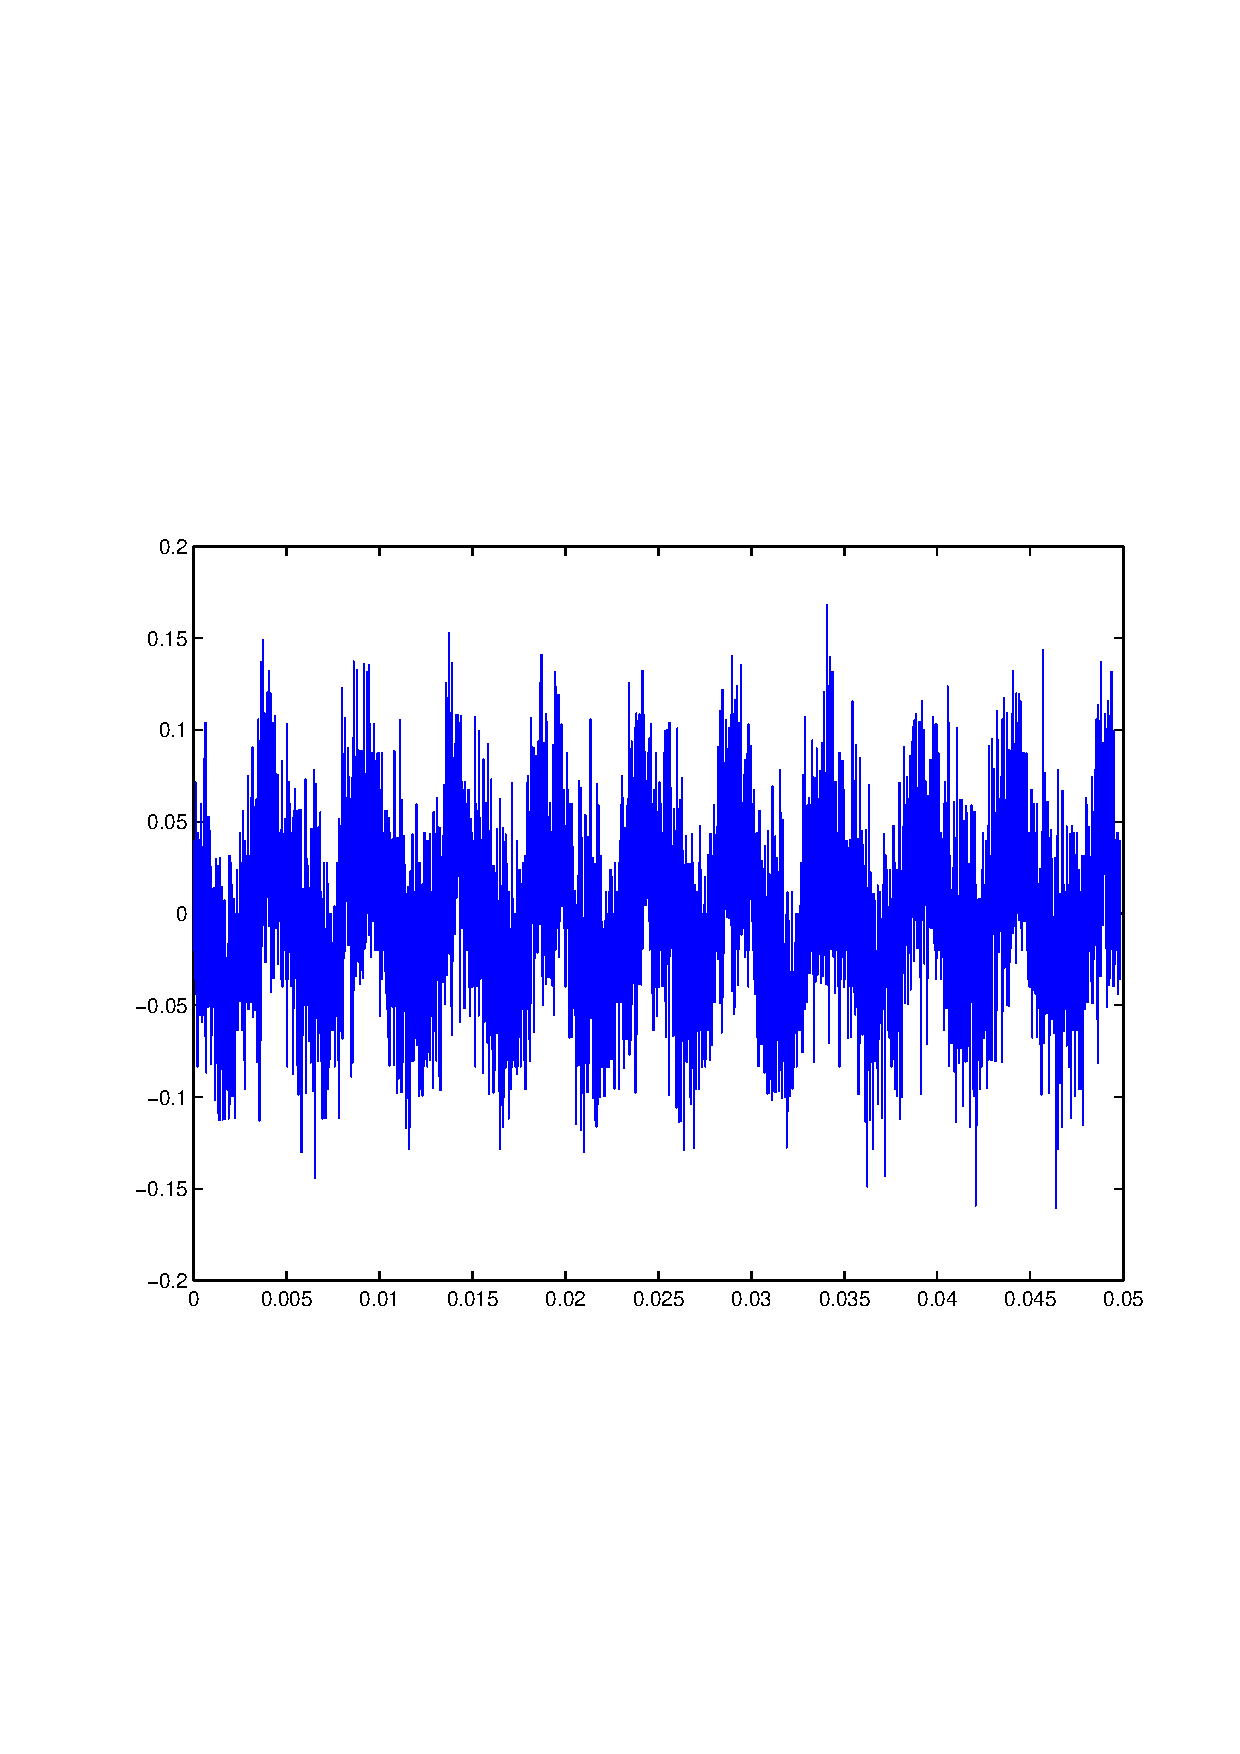
\includegraphics[scale=0.55, trim = 16mm 70mm 16mm 85mm, clip]{Bilder/100kHz_sin_Quantisierungsfehler}
                          \caption{Quantisierungsfehler 100 kHz Sinus}
		                  \label{fig:QuantErr 100 kHz Sinus}
                    \end{figure}
                \end{minipage}
                
                \begin{minipage}{0.6\textwidth}
                    \begin{figure}[H]
                        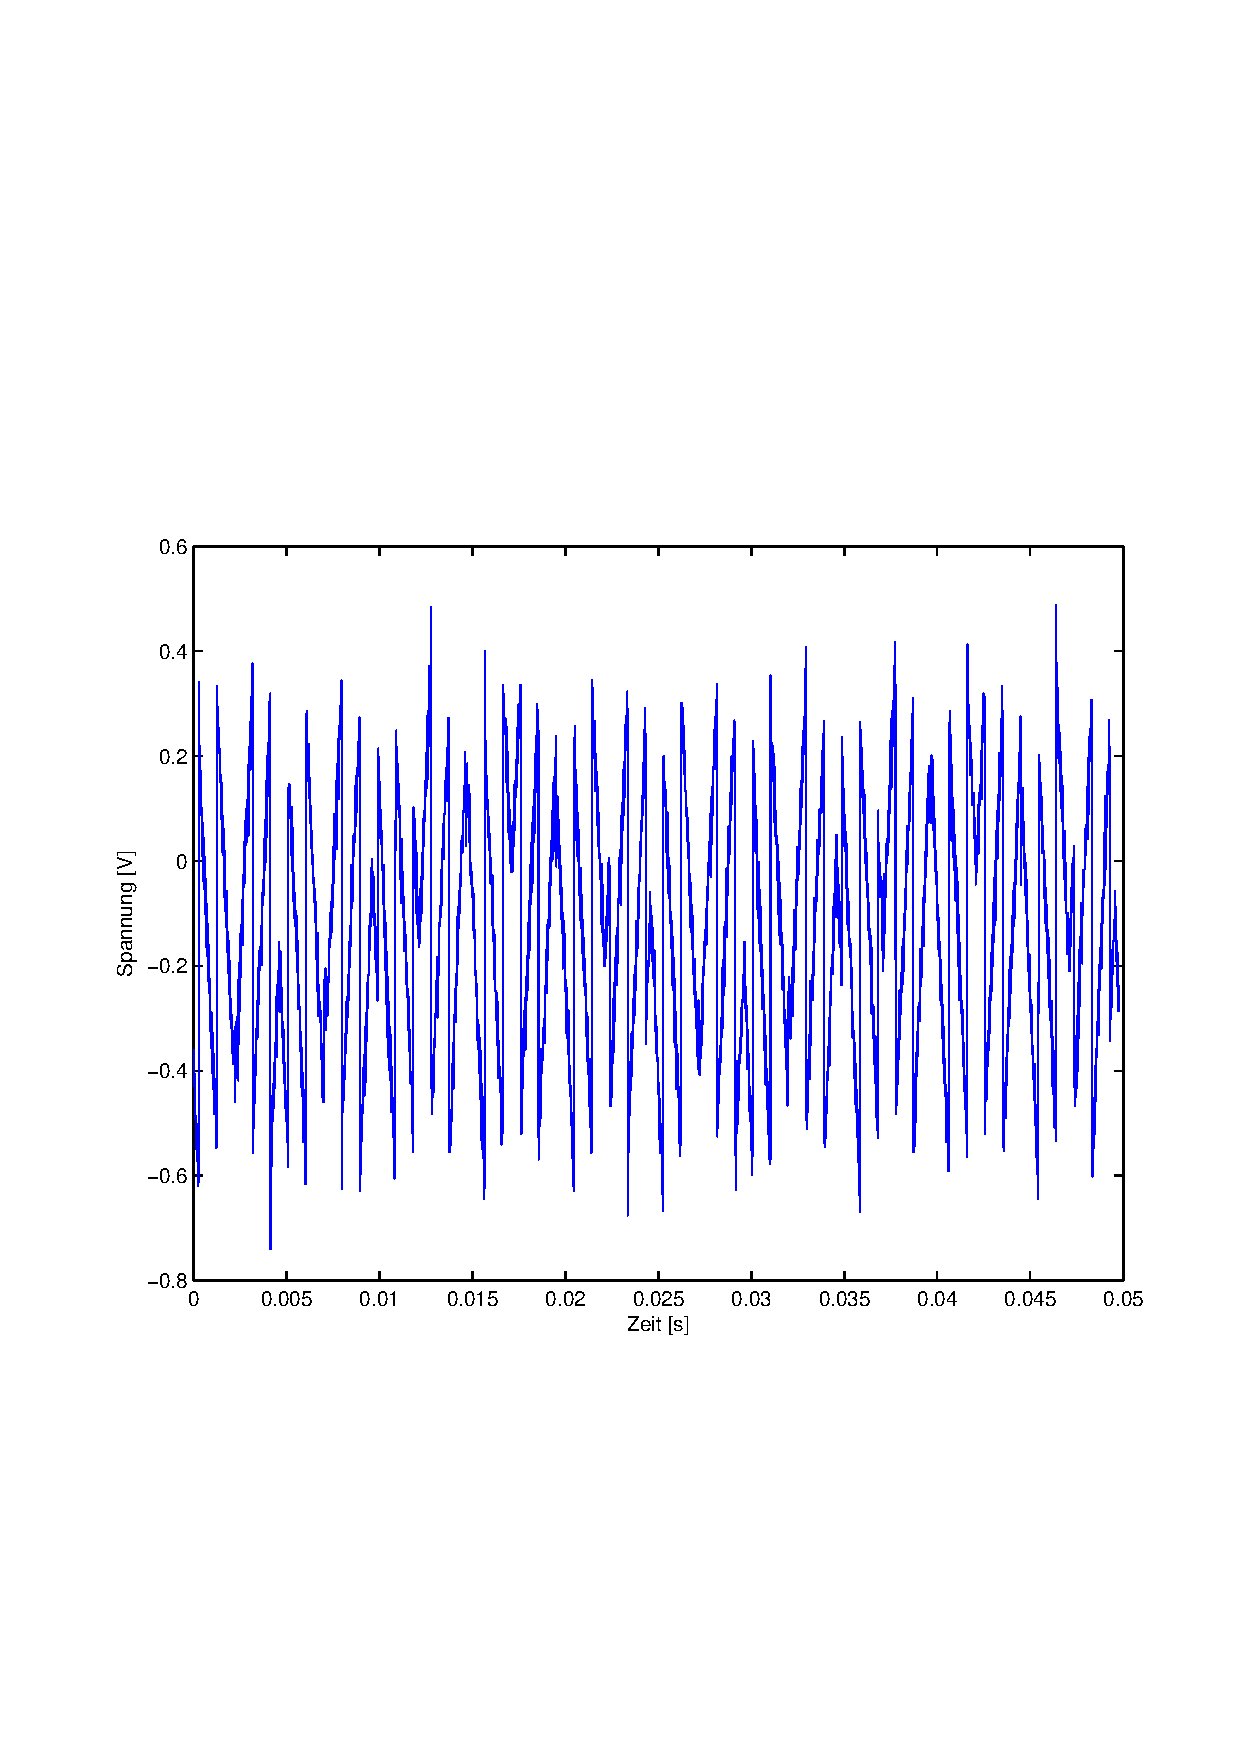
\includegraphics[scale=0.55, trim = 16mm 70mm 16mm 85mm, clip]{Bilder/8kHz_dreieck_Quantisierungsfehler}
                       \caption{Quantisierungsfehler 8 kHz Dreieck}
		              \label{fig:QuantErr 8 kHz Dreieck}
                    \end{figure}
                \end{minipage}
            
            \end{tabular}
            \end{center}
            
            \vspace{2em}
	   	
	   	
	   	
	   	
	   	Für das Leistungsdichtespektrum wird die Autokorrelation des Quantisierungsfehlers mit dem Befehl xcorr aus matlab
	   	gebildet und das Ergebnis dann Fouriertransformiert (Abb.).
	   	
	   	
    	
    	\end{quote}
    
\end{quote}


\end{document}